\section*{Appendix}
\addcontentsline{toc}{section}{Appendix}
\subsection*{Stepper motors specifics}
\addcontentsline{toc}{subsection}{Stepper motors specifics}
% \subsubsection{RA stepper motor}
\begin{minipage}{0.5\textwidth}
    \centering
    \begin{tabular}{cc}
        \textbf{17HM15-0904S stepper motor}&\\
        Electronics&\\
        \hline
        Manufacturer code & 17HM15-0904S\\
        Engine type & bipolar\\
        Pitch angle (deg) & 0.9 \\
        Torque (Ncm)& 36\\
        Rated current/phase (A) & 0.9\\
        Phase resistance (Ohm)& 60\\
        Voltage (V)& 5.4\\
        Inductance (mH)& 12 \(\pm\) 20\% (1 kHz)\\
         & \\
        Physical specifications&\\
        \hline
        Frame dimensions (mm\(^2\))& 42x42 \\
        Body length (mm)& 40 \\
        Shaft diameter (mm)& 5 \\
        Stem length (mm)& 22 \\
        D-cut length (mm)& 15 \\
        Number of cables & 4\\
        Lead number (mm)& 300 \\
        Weight (g) & 280\\
        \hline
    \end{tabular}
    \captionof{table}{Nema 17 (0.9A) stepper motor specifics.}
    \label{tab:nema_17_specifics}
\end{minipage}

% \subsubsection{DEC stepper motor}

\begin{minipage}{0.5\textwidth}
    \centering
    \begin{tabular}{cc}
        \textbf{17HM19-2004S1 stepper motor}&\\
        Electronics&\\
        \hline
        Manufacturer code & 17HM19-2004S1\\
        Engine type & bipolar\\
        Pitch angle (deg) & 0.9 \\
        Torque (Ncm)& 46\\
        Rated current (A) & 2\\
        Phase resistance (Ohm)& 1.4\\
        Voltage (V)& 2.8\\
        Inductance (mH)& 4\\
         & \\
        Physical specifications&\\
        \hline
        Frame dimensions (mm\(^2\))& 42x42 \\
        Body length (mm)& 48 \\
        Shaft diameter (mm)& 5 \\
        Stem length (mm)& 24 \\
        D-cut length (mm)& 24 \\
        Number of cables & 4\\
        Lead number (mm)& 500 \\
        Weight (g) & 370\\
        \hline
    \end{tabular}
    \captionof{table}{Nema 17 (2A) stepper motor specifics.}
    \label{tab:nema_17_specifics_2}
\end{minipage}

% \subsubsection{Focuser stepper motor}
\begin{minipage}{0.5\textwidth}
    \centering
    \begin{tabular}{cc}
        \textbf{11HS12-0674S stepper motor}&\\
        Electronics&\\
        \hline
        Manufacturer code & 11HS12-0674S\\
        Engine type & bipolar\\
        Pitch angle (deg) & 1.8 \\
        Torque (Ncm)& 7\\
        Rated current (A) & 0.67\\
        Phase resistance (Ohm)& 5.6\\
        Voltage (V)& 3.8\\
        Inductance (mH)& 4.2\\
         & \\
        Physical specifications&\\
        \hline
        Frame dimensions (mm\(^2\))& 28x28 \\
        Body length (mm)& 31.5 \\
        Shaft diameter (mm)& 5 \\
        Stem length (mm)& 20 \\
        Number of cables & 4\\
        Lead number (mm)& 300 \\
        Weight (g) & 110\\
        \hline
    \end{tabular}
    \captionof{table}{Nema 11 stepper motor for the focuser motion specifics.}
    \label{tab:nema_11_specifics}
\end{minipage}

% \subsection*{ESP32 pinout map}
% \addcontentsline{toc}{subsection}{ESP32 pinout map}
% \begin{minipage}{0.5\textwidth}
%     \centering
%     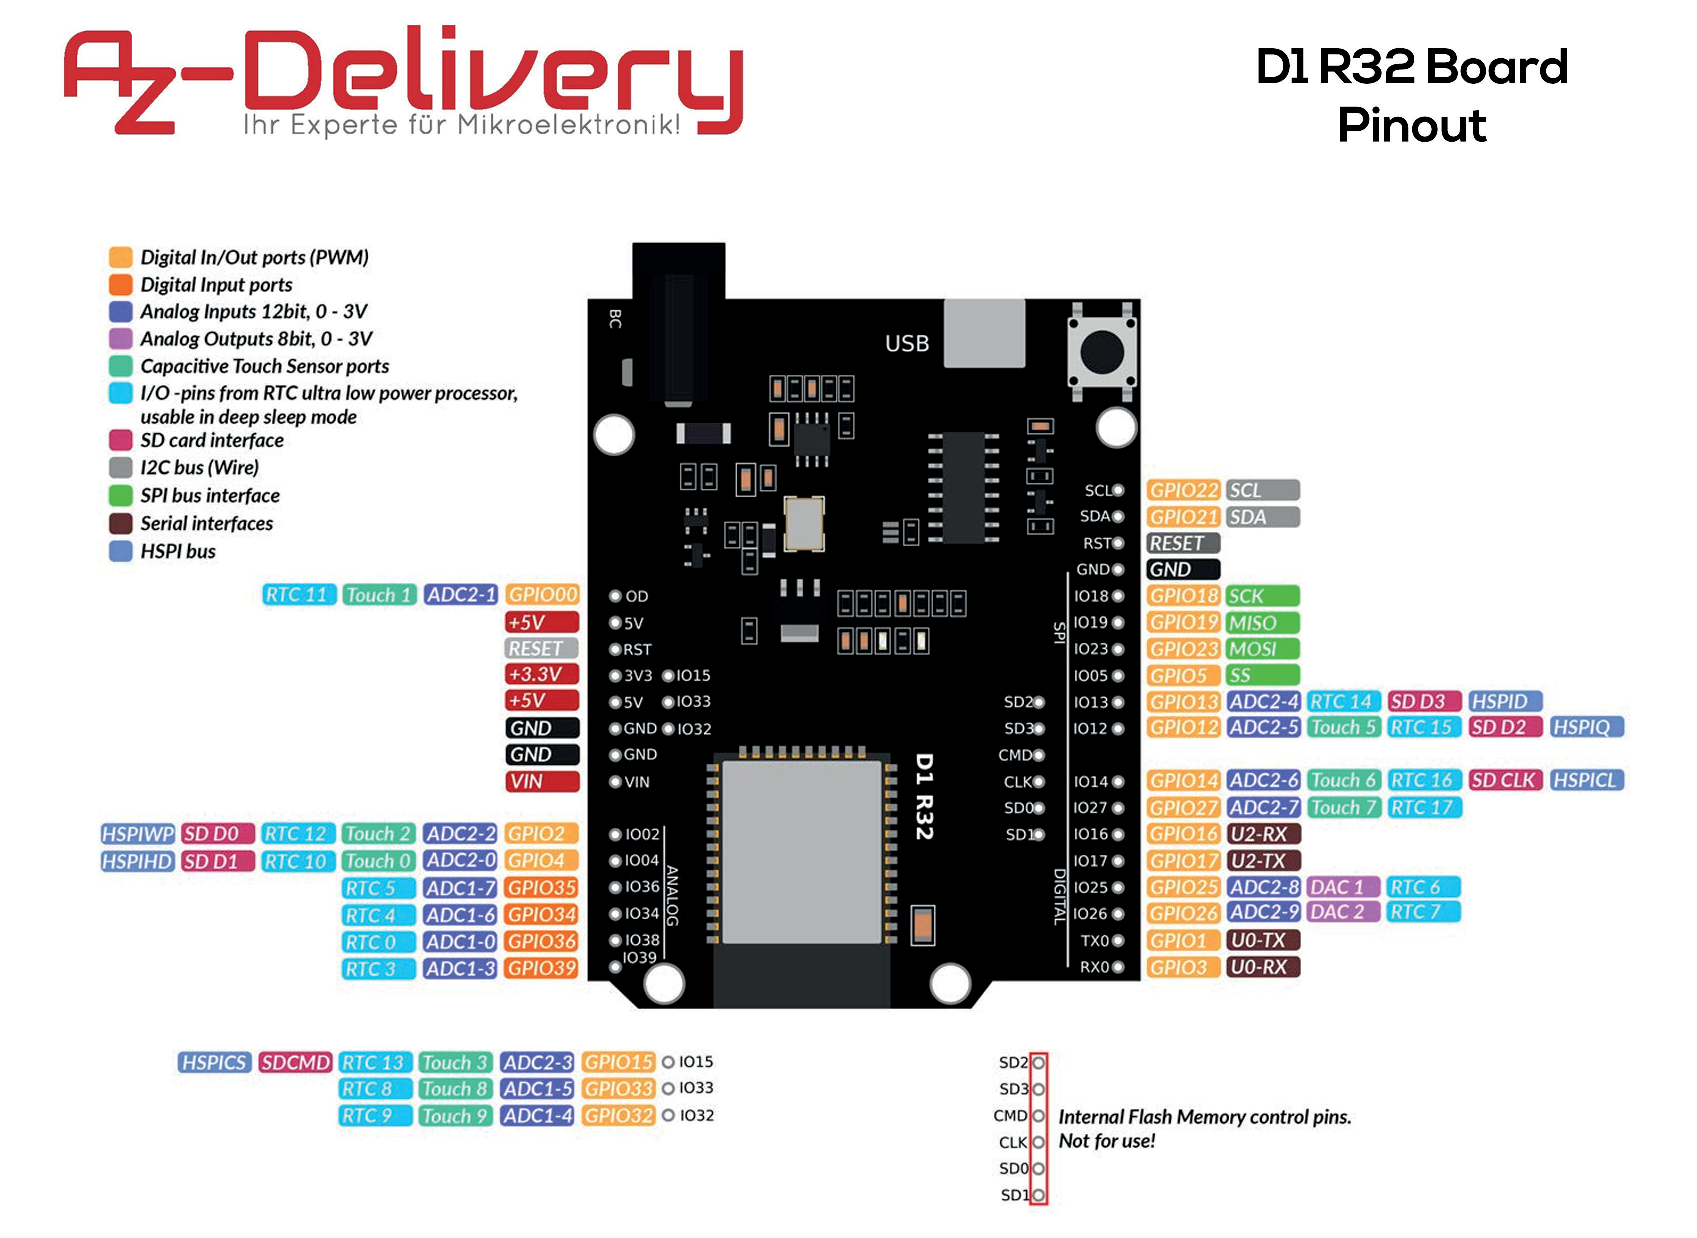
\includegraphics[scale=0.5]{Setup/D1 R32 Board Pinout.pdf}
%     \captionof{figure}{ESP32 pinout map}
%     \label{fig:esp32-pinout-map}
% \end{minipage}

% \subsection*{CNC Shield V3 Schematic}
% \addcontentsline{toc}{subsection}{CNC Shield V3 Schematic}
% \begin{minipage}{0.5\textwidth}
%     \centering
%     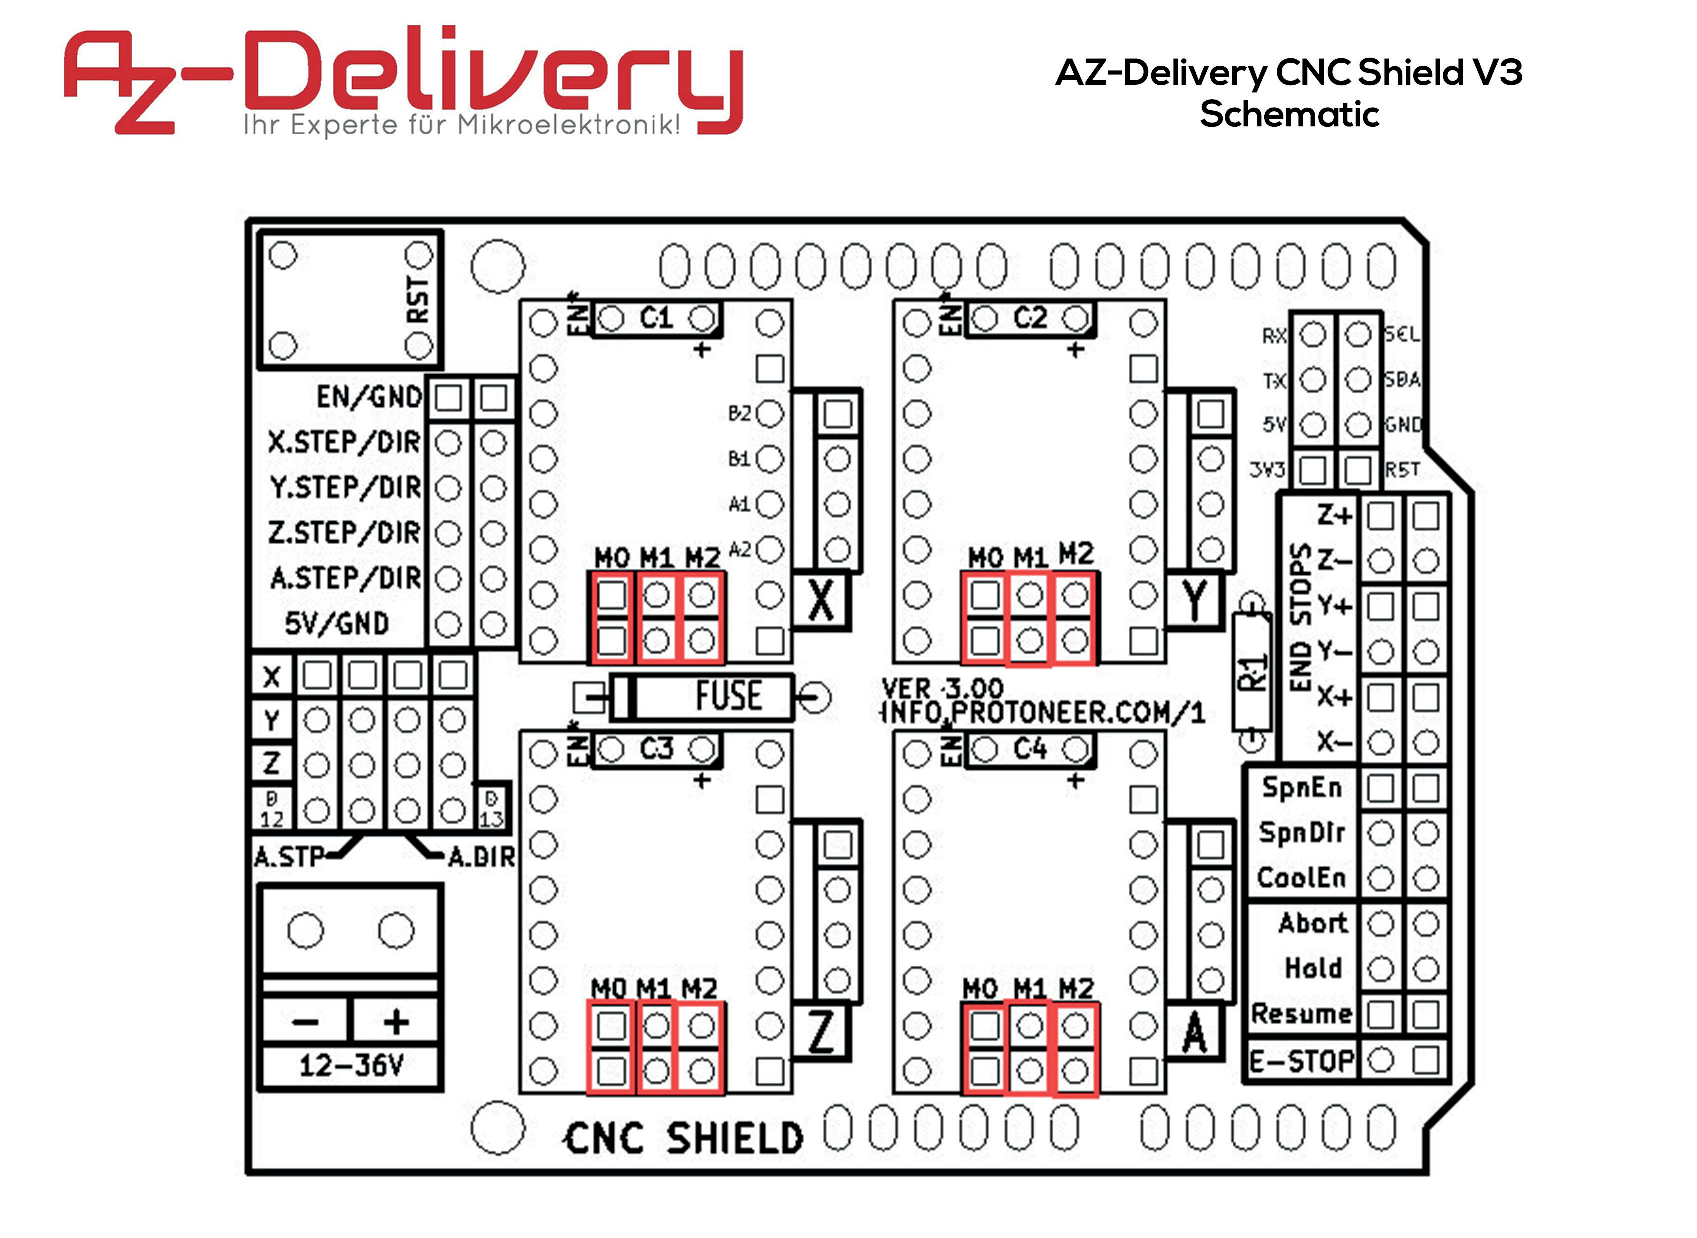
\includegraphics[scale=0.3]{Setup/AZ-Delivery CNC Shield V3 Schematic.pdf}
%     \captionof{figure}{CNC Shield V3 Schematic}
%     \label{fig:cnc3-schematic}
% \end{minipage}

